% !TEX encoding = UTF-8 Unicode
% !TEX root = thesis-ex.tex

This discussion is based on the work in Refs. \cite{Casalderrey-Solana:2014bpa, Hulcher:2017cpt, Casalderrey-Solana:2016jvj} and describes jet quenching using a hybrid strong/weak model. It uses perturbative QCD to describe the weakly coupled hard process of jet production and holographic calculations of the energy loss of energetic probes to model the strong coupling between the probe and the plasma \cite{Chesler:2015nqz, Chesler:2014jva}. This is a combination of approaches that focus on the following extreme limits: a weakly coupled system at unrealistically high temperatures that can be treated perturbatively \cite{Jacobs:2004qv, Majumder:2010qh} and a system where the coupling constant is large at all energy scales and Gauge/string duality is applicable \cite{CasalderreySolana:2011us}.

In this model, the jet evolves in space time with the lifetime of the parton in the shower being given by \cite{CasalderreySolana:2011gx}.  

\begin{align}
\tau = 2 \frac{E}{Q^2}
\end{align}
where $Q$ is its virtuality and $E$ its energy. This evolution is unaffected before the proper time at which the plasma hydrodynamizes, $\tau_{\text{hydro}} = 0.6$ fm. After this time, the jet-plasma interaction comes into play and the fragments evolve with the energy loss as:

\begin{align}
\frac{1}{E_{\mathrm{in}}} \frac{dE}{dx} = -\frac{4}{\pi} \frac{x^2}{x_{\mathrm{stop}}^2} \frac{1}{\sqrt{x_{\mathrm{stop}}^2 - x^2}}
\end{align}
where $E_{\mathrm{in}}$ is the initial energy of the parton prior to any quenching and $x_{\mathrm{stop}}$ is its stopping distance (jet thermalization distance). The stopping distance can be written as:

\begin{align}
x_\mathrm{stop} = \frac{1}{2\kappa_\mathrm{sc}} \frac{E_\mathrm{in}^{1/3}}{T^{4/3}}
\end{align}
where $\kappa_\mathrm{sc}$ is a dimensionless free parameter associated to the strong coupling and is used to fit to the data. The energy loss is characterized by the strong  $x^2$ dependence for $x \ll x_\mathrm{stop}$. Furthermore, when $x$ is comparable to $x_\mathrm{stop}$, $dE/dx$ depends nontrivially on $E_\mathrm{in}$ and $x$, diverging for $x\rightarrow x_\mathrm{stop}$ and $E\rightarrow0$. The shower is then embedded into a hydrodynamic description of the QGP from Ref. \cite{Hirano:2010je}, and the energy loss expressions are integrated for each parton, from the time it is produced to the time that it splits. The splitting probabilities are taken to be independent of the medium, depending only on the initial energy of the daughter partons. These further lose energy as they propagate through the QGP and split. Then the total energy lost by a parton is dependent on the history of splitting and propagation of its parents, grandparents and so on and so forth. 

The partons further experience kicks transverse to their direction of motion, a phenomena called transverse momentum broadening. This effect is mainly experienced by softer partons that are much more affected by the angular narrowing effects of energy loss, making most measured observables insensitive to the size of this kick. This is directly related to wider jets losing more energy than narrower ones. The wake left in the medium from the partons depositing momentum in the QGP as they propagate through it lends a non-trivial impact to the model predictions. This wake moves in the direction of the jet and is impossible to separate out in experiments, making its inclusion to any model vital. This wake results in a perturbation to the hydrodynamic background, resulting in corrections to the final state hadron spectra. This effect is particularly important for jet substructure observables like jet fragmentation and jet shapes \cite{Casalderrey-Solana:2016jvj}.

A screening effect recently included in the hybrid model is based considering the resolving power of the QGP \cite{Hulcher:2017cpt}. As depicted in Figure~\ref{fig:hm_lres}, the QGP will only resolve daughter partons of a splitting after they are separated by a certain distance $L_\mathrm{res}$. It is only after they are resolved that they will be allowed them to lose energy independent of each other. This delayed quenching results in an enhancement of softer partons at larger angles from the jet axis compared to the case where the daughter partons are resolved immediately after they split from the parent parton. The \Lres\ parameter has the constraint $ 1/(\pi T) < \Lres < 2 /(\pt T$ based on the Debye screening length for the plasma, i.e. the length at which the QGP is able to resolve and screen color charges.

%The effects of including the \Lres parameter in the context of jet observables are discussed below.

\begin{figure}[htbp]
\begin{center}
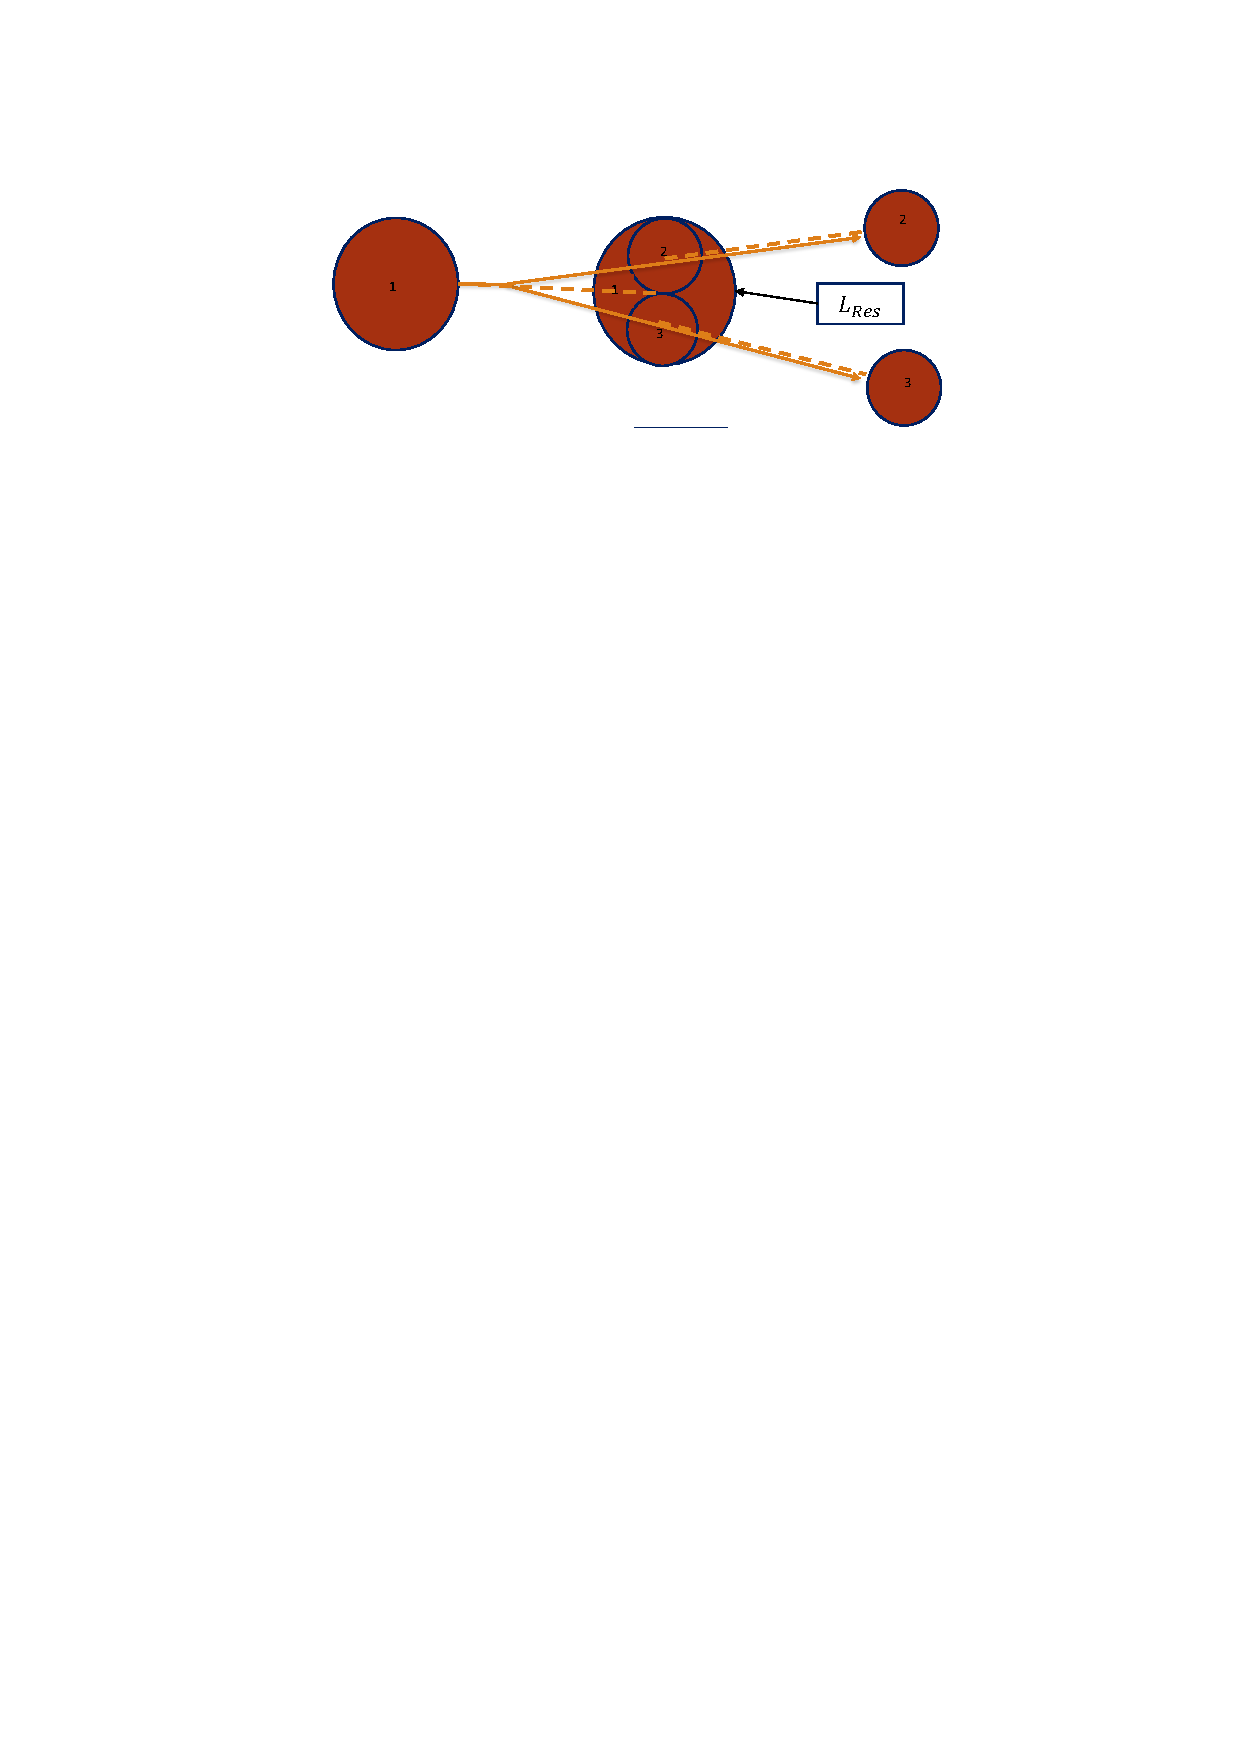
\includegraphics[width=0.55\textwidth]{figures/jetMeasurements/HM_lres}
\caption{A schematic illustrating the resolving power of the QGP. The daughter partons $2$ and $3$ that come from $1$ need to be separated by \Lres\ before they are treated individually by the plasma. Prior to that separation, they are treated as one effective parton. Figure taken from \cite{Hulcher:2017cpt}.}
\label{fig:hm_lres}
\end{center}
\end{figure}


The free parameter $\kappa_\mathrm{sc}$ is determined by fitting to jet \RAA\ data from CMS \cite{Khachatryan:2016jfl} as shown in Figure~\ref{fig:hm_fitting}. It can be seen that including the \Lres\ parameter does not really affect the jet \RAA\ prediction. The dependence of the \RAA\ on the size of the jet radius can be seen. This is consistent with the expectation that wider jets lose more energy.

\begin{figure}[htbp]
\begin{center}
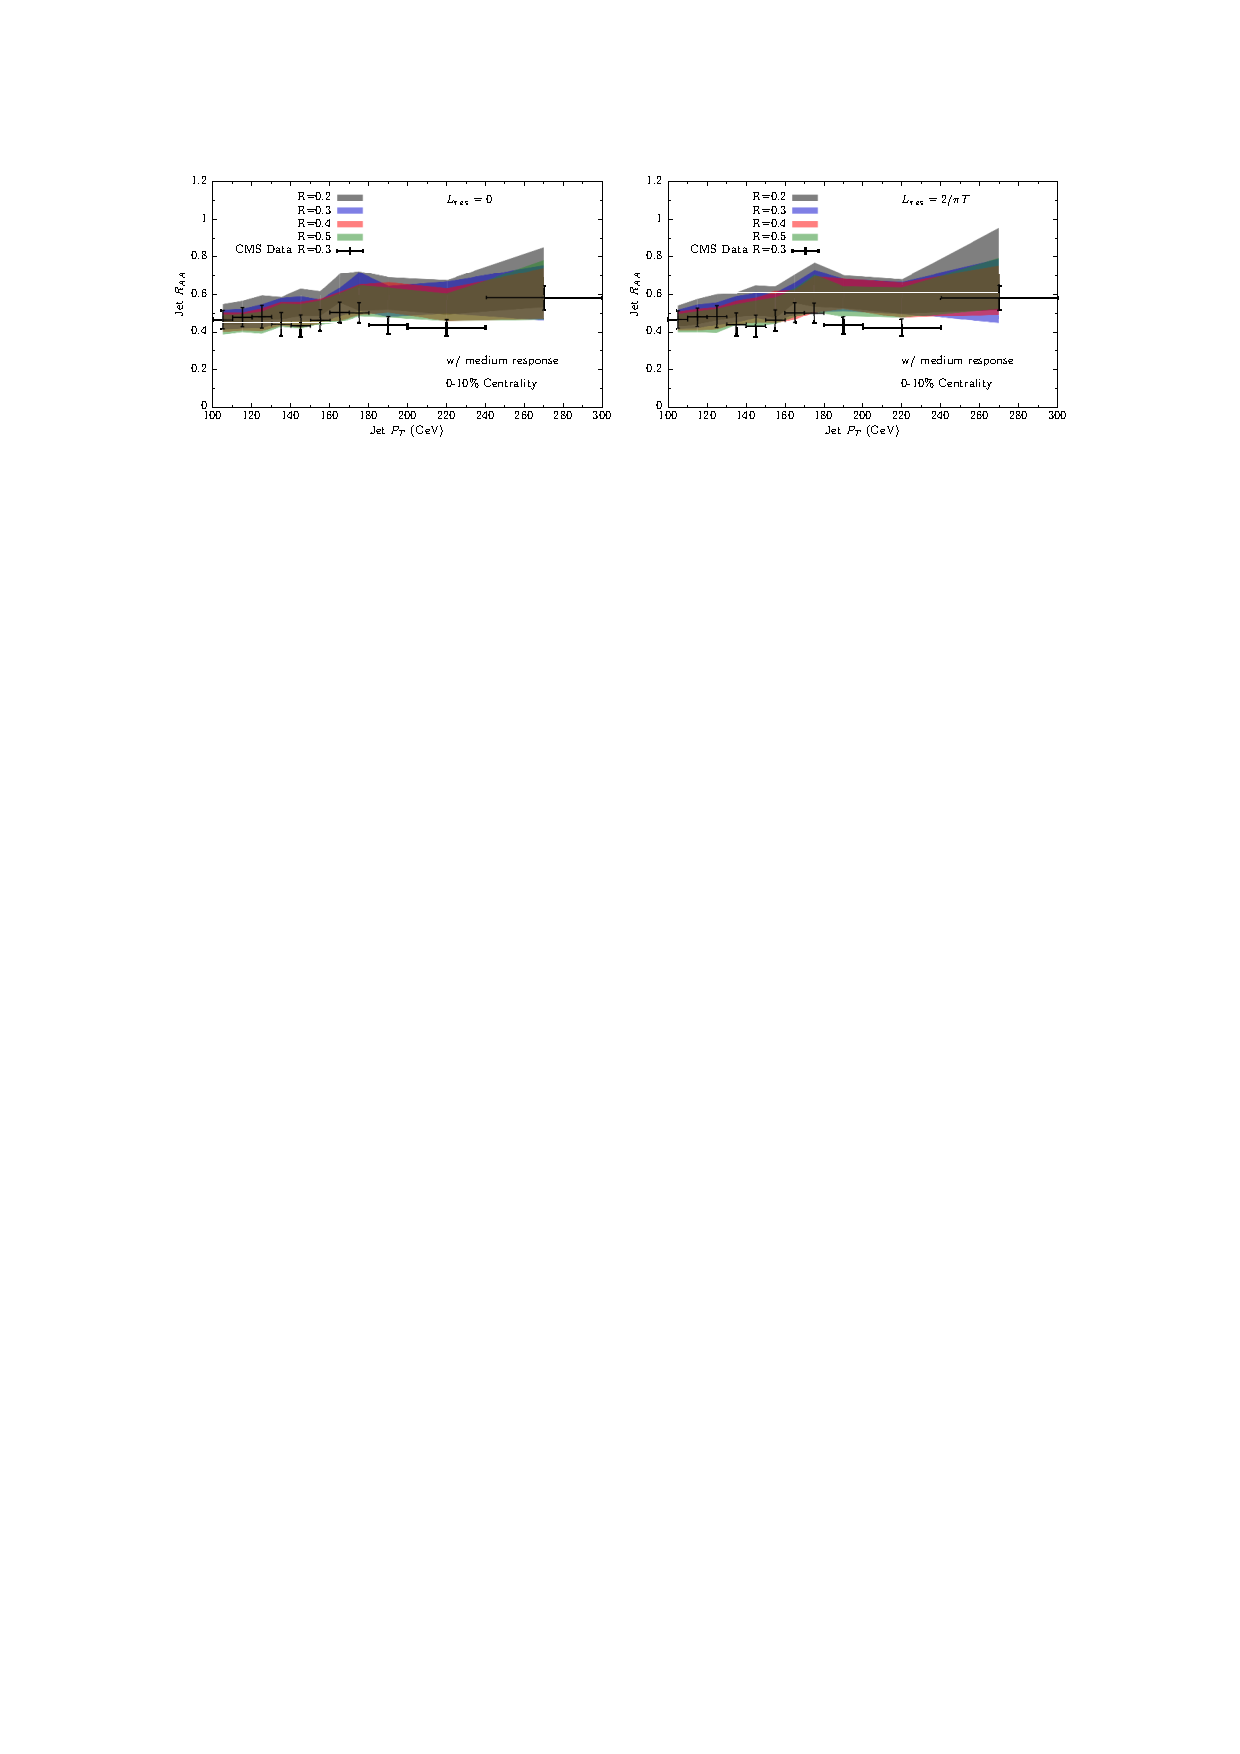
\includegraphics[width=1\textwidth]{figures/jetMeasurements/HM_raa}
\caption{The hybrid model without (left) and with (right) the \Lres\ parameter, compared to the jet \RAA\ as a function of jet \pt\ in two centrality intervals as measured in Ref. \cite{Khachatryan:2016jfl}. The different colors correspond to different jet radii. The Hybrid Model is fit to the 100--110 GeV point from the data, giving rise to the colored bands. Figure taken from \cite{Hulcher:2017cpt}. }
\label{fig:hm_fitting}
\end{center}
\end{figure}

Fixing the $\kappa_\mathrm{sc}$ parameter allows for predictions of other jet measurements like jet fragmentation and jet shape. Figures~\ref{fig:hm_ff} and \ref{fig:hm_jetshape} show a comparison of the measured and modeled values of the modifications to the jet fragmentation and jet shape respectively.  The model has also been compared to measurements done by ATLAS, ALICE, and STAR \cite{2013220, Abelev:2013kqa, RUSNAK:2014xfa} \cite{}


\begin{figure}
\begin{subfigure}{1\textwidth}
  \centering
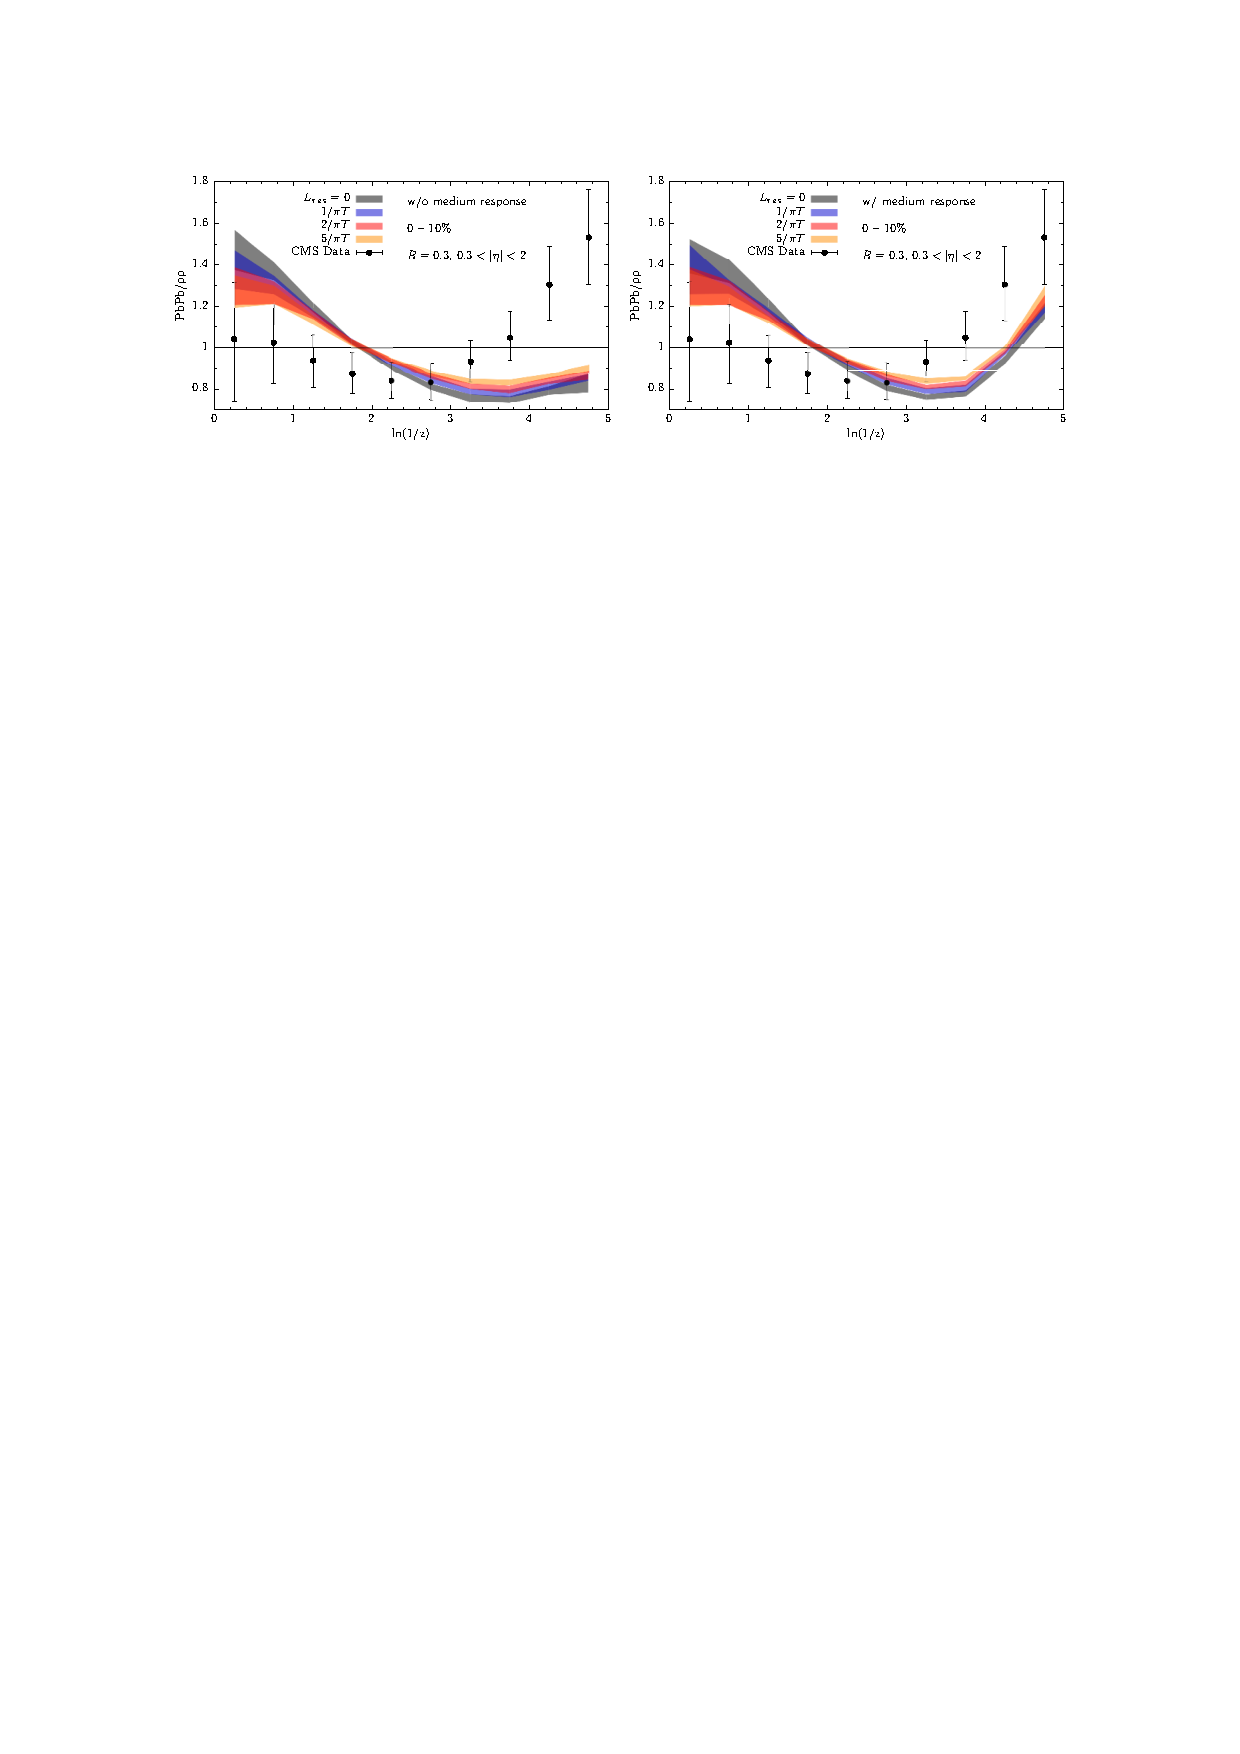
\includegraphics[width=1\textwidth]{figures/jetMeasurements/HM_FF}
\caption{The modification to the jet fragmentation from \pp\ to \pbpb\ as a function of $\ln(1/z)$ as measured in Ref. \cite{Chatrchyan:2014ava} compared to the predictions of the hybrid model. The predictions are shown without (left) and with (right) the effect of the wake from the QGP responding to the jet. The different colors correspond to different \Lres\ parameters. Figure taken from \cite{Hulcher:2017cpt}. }
\label{fig:hm_ff}
\end{subfigure} \\ \\ \\
\begin{subfigure}{1\textwidth}
  \centering
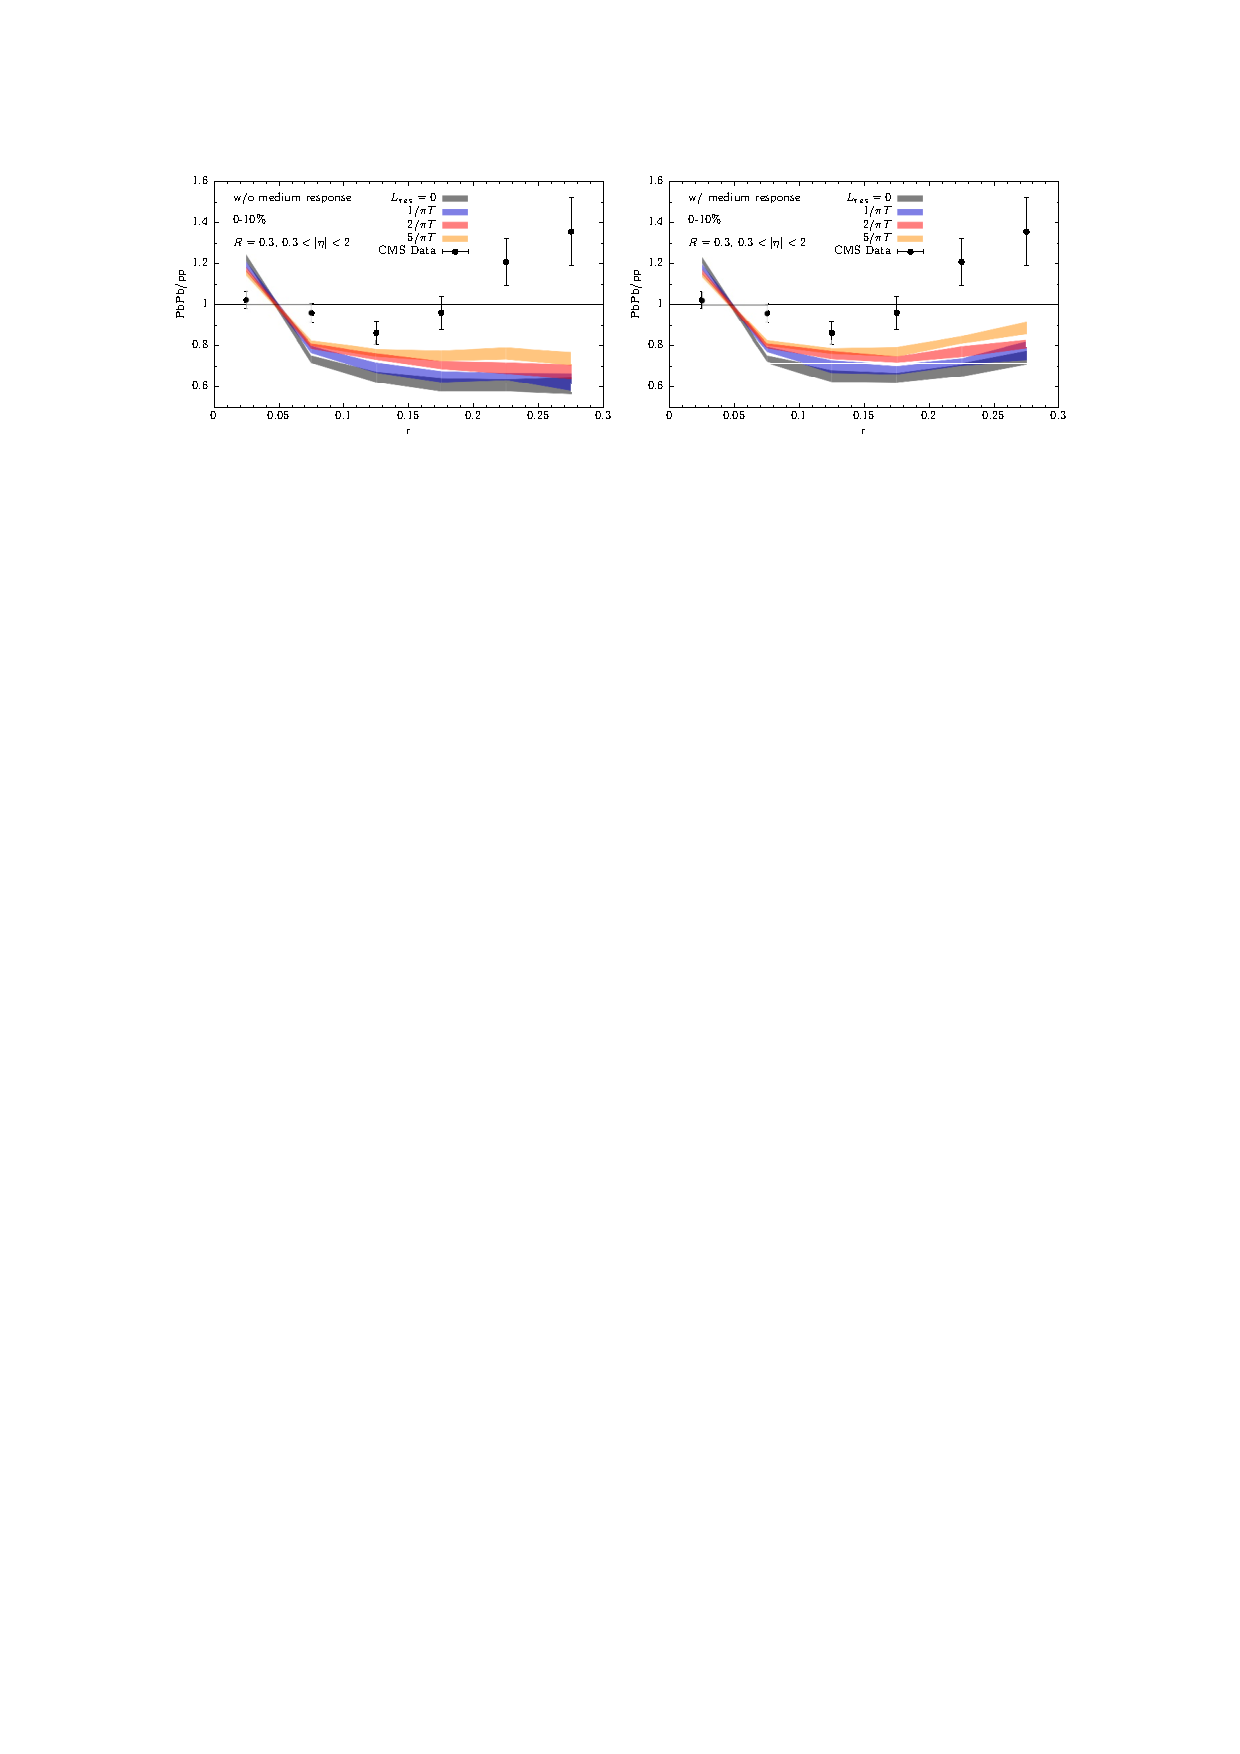
\includegraphics[width=1\textwidth]{figures/jetMeasurements/HM_jetShape}
\caption{The modification to the jet shape from \pp\ to \pbpb\ as a function of $r$ as measured in Ref. \cite{Chatrchyan:2013kwa} compared to the predictions of the hybrid model. The predictions are shown without (left) and with (right) the effect of the wake from the QGP responding to the jet. The different colors correspond to different \Lres\ parameters. Figure taken from \cite{Hulcher:2017cpt}. }
\label{fig:hm_jetshape}
\end{subfigure}
\caption{A comparison of measured data, MC, and the analytic calculation of the EQ model. Figure taken from \cite{Spousta:2015fca}}
\label{fig:HM_modification}
\end{figure}


Here it can be seen that adding a medium response and a non-zero \Lres\ parameter affects the prediction. While the hard fragments (see Figure~\ref{}) are unaffected by the medium response, including the soft particles from the wake compensates some of the suppression of soft fragments in \pbpb\ compared to \pp\ collisions. Moreover, including the \Lres\ parameter further compensates the suppression for soft fragments, while reducing the enhancement of the hard fragments. This is a result of allowing more hadrons carrying a smaller fraction of the jet energy (low $z$, high ($\ln(1/z)$) to survive into the final state. The jet shape observable (see Figure~\ref{}) quantifies the radial distribution of energy in terms of annuli around the jet axis. It can be seen that introducing the \Lres\ parameter enhances the probability to find final state hadrons at larger distances from the jet axis. The jet core ($r < 0.05$) is also affected, with the depletion only slowly evolving with an increasing \Lres. One must be careful before making conclusions though, since these modifications are made between jets that are quenched (in \pbpb\ ) and unquenched (in \pp\ ). Taking into account the fact that wider jets lose more energy and that the jet spectrum rapidly falls off, there is a bias for finding narrower quenched jets than unquenched jets. This makes the jet shape after quenching narrower in \pbpb\ compared to \pp. While the model is not fully able to capture the features in the data, including the medium response moves it in the correct direction. It can be suggested that the model is missing a description of the medium induced modification to the hadronization process or that the wakes in the plasma are not equilibrating.









